\documentclass[conference]{IEEEtran}
\IEEEoverridecommandlockouts
% The preceding line is only needed to identify funding in the first footnote. If that is unneeded, please comment it out.
\usepackage{cite}
\usepackage{amsmath,amssymb,amsfonts}
\usepackage{algorithmic}
\usepackage{graphicx}
\usepackage{textcomp}
\usepackage{xcolor}
\usepackage{array}
\usepackage{url}
\def\BibTeX{{\rm B\kern-.05em{\sc i\kern-.025em b}\kern-.08em
    T\kern-.1667em\lower.7ex\hbox{E}\kern-.125emX}}
\begin{document}

\title{Which Words Make a Reel Travel?\\A Within-Creator Look at Portuguese Reels}

\author{\IEEEauthorblockN{Max Christian Metzger Egger}
\IEEEauthorblockA{\textit{Natural Language Processing (2026s2)} \\
\textit{Insper}\\
S\~ao Paulo, Brazil}
}

\maketitle

\section{Introduction}
People who write Instagram copy in Portuguese follow rules of thumb: ask a question in the hook, talk to \textit{voc\^e}, put a number up front.
Most of this advice comes from English-language marketing and has never been checked on Portuguese short videos.
Checking it is hard because a big creator's Reels get more views whatever they say, so comparing creators mostly measures audience size.

Earlier work solved this by comparing a message only with similar messages.
Tan et al.~\cite{tan2014} paired tweets by the same author on the same link and asked which one was retweeted more: people got 61.3\% of the pairs right and their best model 65.6\%.
Hessel et al.~\cite{hessel2017} compared Reddit posts only with posts from the same community and time, and found that context matters as much as content.
Berger and Milkman~\cite{berger2012} showed that news articles that trigger strong emotions are shared more.
I found no study of this kind for Portuguese, or for the copy of short videos.

Follower count is the strongest predictor of a Reel's views, and the platform's algorithm adds its own bias, so I decided to compare each creator only with themself: which of their own Reels did better than usual, and what was different in the text?
The goal is the measurable one from Tan et al.: pick the more viral of two Reels by the same creator more often than chance, and get close to their 61\% (people) and 66\% (model).
The project also has an educator side: copy tips for each sector, a notebook that lets any creator run the analysis on their own profile, and a test of whether the tips help people.

\section{How the project was done}
I designed the project and made the main decisions; I used AI (Claude, by Anthropic) to write and run the code (Table~\ref{tab:who}).

\begin{table}[htbp]
\caption{Who did what}
\begin{center}
\footnotesize
\begin{tabular}{>{\raggedright\arraybackslash}p{0.60\columnwidth}>{\raggedright\arraybackslash}p{0.28\columnwidth}}
\hline
Research question, Portuguese, comparing each creator only with themself & me \\
Sectors, creators and how to collect the data (free, with my own Instagram account) & me \\
Methods from the course, the ``viral'' metric and the analyses & me \\
Human test design and recruiting the participants & me \\
Writing and running the code: data collection, transcription, experiments, test page & AI \\
Report text & me, with AI grammatical and structural revision \\
\hline
\end{tabular}
\label{tab:who}
\end{center}
\end{table}

\section{Data and Methods}
\textbf{Data.} I picked nine creators in five sectors: AI (@odanilogato, @beprecht), hair (@eduardomulleroficial, @brunooliver), sales (@leandrobranquinho, @thiagoconceroficial), trading (@portstrader, @cafecomferri) and sports (@tiagoleifert).
To avoid paying for a scraper, the AI browsed their public Reels pages in Chrome on my personal account, slowly and without liking or following anything, and saved views, likes, comments, caption and date.
This gave 1,005 Reels posted from 2019 to 2026.
The speech was transcribed for free on my laptop with Whisper~\cite{whisper}; 874 Reels have speech, and the \emph{opening} is what is said in the first five seconds.

\textbf{What ``viral'' means.} A Reel's \emph{lift} is its log views minus the median log views of the same creator's 10 Reels before and 10 after it.
This compares a Reel only with its neighbours, so audience size and follower growth drop out.
For each creator, the oldest 70\% of Reels are used for training and the newest 30\% for testing, so no model sees the future.
A test pair is two Reels by the same creator, posted at most 14 days apart, where one got at least 1.5 times the views (136 test pairs).

\textbf{Methods.} All come from the course, each answering one question.
TF-IDF with logistic regression asks whether the words predict the winner, and its probabilities rank the words.
Regular expressions count copy devices (questions, numbers, calls to action, talking to \textit{voc\^e}), and the Brazilian version~\cite{anewbr} of the ANEW lexicon used in class measures emotion; both test the popular tips directly, together with the perplexity of each opening under a bigram model of the creator's other openings (PPL), which measures how formulaic it is.
Frozen BERT embeddings, from BERTimbau~\cite{bertimbau}, the Portuguese version of the BERT used in class, check whether a pretrained model sees more than word counts.
Training on one creator and testing on another asks whether the lessons transfer, and LDA topics~\cite{lda} separate wording from subject.
Confidence intervals resample creators, so one creator cannot drive a result.

\textbf{Educational material.} For each sector, a short card lists the words and copy devices that went with each creator's stronger and weaker Reels, with real examples.
A notebook reruns the whole analysis on any creator's own export, since the main lesson is personal.
To check whether the cards teach anything, volunteers judged test pairs before and after reading four tips taken from them.

\section{Results}
\textbf{How much is said in the first five seconds matters more than which words are used.}
In test pairs, the Reel with fewer words in its opening won 63\% of the time ($p=0.003$).
A model that knows only that count and the caption length picks the winner in 66\% of pairs (Fig.~\ref{fig:e3}), level with Tan et al.'s model.
The effect was strongest in sales (80\% of pairs) and trading (69\%), and absent for the one sports creator (45\%, 11 pairs).
Word models also beat chance (TF-IDF 62\%, BERT 58\%), while the copy devices and the emotion scores do not (53\%).
More data would help the word models: TF-IDF went from 58\% with a fifth of the training Reels to 62\% with all of them.

\begin{figure}[htbp]
\centerline{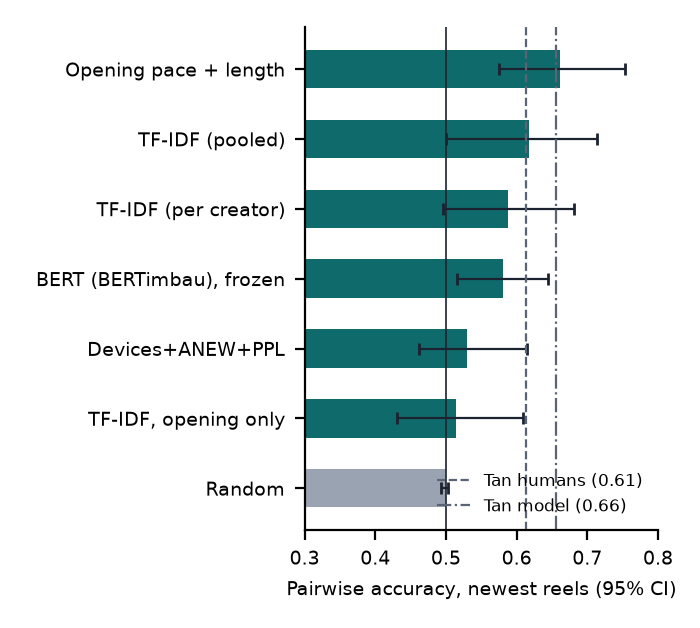
\includegraphics[width=\columnwidth]{fig_e3_pairwise_accuracy.png}}
\caption{How often each model picks the more viral of two Reels by the same creator, on the newest 30\% of Reels, with 95\% confidence intervals. Dashed lines: Tan et al.~\cite{tan2014} on tweets.}
\label{fig:e3}
\end{figure}

\textbf{The popular tips do not hold up.} No copy device, including questions and talking to \textit{voc\^e}, helps consistently across creators.
The words that most clearly go with weaker Reels are promotions (\textit{loja virtual}, \textit{de desconto}) and course-style promises (\textit{voc\^e vai}, \textit{voc\^e aprende}).

\textbf{What works is personal.} A model trained on one creator does no better than chance on a creator from another sector (50\%, against 59\% on the same creator), no viral word is shared by two creators, and topics alone are at chance (49\%).

\textbf{Human test.} Fourteen volunteers judged 16 test pairs, 8 before and 8 after reading four tips.
They got 56\% right, below the 66\% of the opening model, and the tips did not help (58\% before, 54\% after; the 95\% interval rules out a gain above 6 points).

\section{Conclusion}
Comparing each creator with themself works: it removes audience size and still finds a signal that a model can use as well as Tan et al.\ did on tweets.
The signal is not the one marketers talk about.
The common hook tips did not hold up; what did is saying less in the first seconds, and beyond that each creator's winning words are their own.
For creators, the practical lesson is to compare yourself with yourself, which the notebook makes easy.
Code, results, cards, notebook and test page: \url{https://github.com/max-egger-syno/reels-copy-nlp}.

The limits are real: about 110 Reels per creator, one sports creator, views as the only measure, and correlation only, since a slower opening may stand for editing style.
We also found and fixed mistakes along the way: the test page first showed every participant the same order, and the tips came from partial data, before the opening result was known.
What I learned is that, with AI writing and running the code, modeling becomes much easier, so the most important work moves to defining the question and the parameters: what counts as viral, what to compare with what, and how to test it.

\begin{thebibliography}{00}
\bibitem{tan2014} C. Tan, L. Lee, and B. Pang, ``The effect of wording on message propagation: Topic- and author-controlled natural experiments on Twitter,'' in Proc. ACL, 2014, pp. 175--185.
\bibitem{hessel2017} J. Hessel, L. Lee, and D. Mimno, ``Cats and captions vs. creators and the clock: Comparing multimodal content to context in predicting relative popularity,'' in Proc. WWW, 2017, pp. 927--936.
\bibitem{berger2012} J. Berger and K. L. Milkman, ``What makes online content viral?'' J. Marketing Research, vol. 49, no. 2, pp. 192--205, 2012.
\bibitem{anewbr} C. H. Kristensen, C. F. A. Gomes, A. R. Justo, and K. Vieira, ``Normas brasileiras para o Affective Norms for English Words,'' Trends Psychiatry Psychother., vol. 33, no. 3, pp. 135--146, 2011.
\bibitem{bertimbau} F. Souza, R. Nogueira, and R. Lotufo, ``BERTimbau: Pretrained BERT models for Brazilian Portuguese,'' in Proc. BRACIS, 2020, pp. 403--417.
\bibitem{lda} D. M. Blei, A. Y. Ng, and M. I. Jordan, ``Latent Dirichlet allocation,'' J. Machine Learning Research, vol. 3, pp. 993--1022, 2003.
\bibitem{whisper} A. Radford et al., ``Robust speech recognition via large-scale weak supervision,'' in Proc. ICML, 2023, pp. 28492--28518.
\end{thebibliography}

\end{document}
